\documentclass[conference]{IEEEtran}
\IEEEoverridecommandlockouts
% The preceding line is only needed to identify funding in the first footnote. If that is unneeded, please comment it out.
\usepackage{cite}
\usepackage{amsmath,amssymb,amsfonts}
\usepackage{graphicx}
\usepackage{textcomp}
\usepackage{enumitem}
\usepackage{xcolor}
\usepackage{times}
\usepackage{siunitx}
\usepackage{latexsym}
\usepackage{hyperref}
\hypersetup{colorlinks=true,linkcolor=black,citecolor=blue,filecolor=black,urlcolor=blue}
\usepackage{algpseudocode}
\usepackage{algorithm}
\usepackage{caption}
\usepackage{subcaption}

\newcommand{\TG}[1]{\color{blue}From Tristan: #1 \color{black}}

\algnewcommand\algorithmicforeach{\textbf{for each}}
\algdef{S}[FOR]{ForEach}[1]{\algorithmicforeach\ #1\ \algorithmicdo}
\def\BibTeX{{\rm B\kern-.05em{\sc i\kern-.025em b}\kern-.08em
    T\kern-.1667em\lower.7ex\hbox{E}\kern-.125emX}}

\begin{document}

\title{A Comparative study of Dask and Spark for neuroimaging pipelines}

\author{Mathieu Dugr\'e, Val\'erie Hayot-Sasson, Tristan Glatard\\
Department of Computer Science and Software Engineering\\
Montr\'eal, Qu\'ebec, Canada
}

\maketitle

\begin{abstract}
% Topic
As the amount of data increases and is easier to access, Big Data processing becomes
critical in neuroimaging.
% Problem
This is an issue as the currently used frameworks are specialized for neuroimaging
and not Big Data concerns. This can lead to performance decrease or limit the
research we can perform.
% Relevance
The usage of Big Data framework is beneficial to this problem. The state-of-the-art
general purpose Big Data framework Spark has its code base written in Scala, while
our laboratory mostly uses Python. This can be problematic since it is harder to port
our pipelines to the framework. Also, theoretically, it leads to performance decrease.

% Approach
We propose to use Dask since it provides native Python parallelism to pipelines while
providing support to familiar API from the Python's scientific ecosystem.
Unfortunately, there are few comparisons between Spark and Dask; especially in
neuroimaging. Moreover, these studies were done when Dask was still an immature
framework which makes those studies unfair nowadays. This is our motivation to
compare the latest version of Dask with Spark.
% Methods (one sentence)
To evaluate the frameworks, we focus on their performance and their scheduler.

% Key Impact
Our study demonstrates the potential of using Dask as the framework to build
neuroimaging pipelines.
\end{abstract}

\begin{IEEEkeywords}
Big Data, Dask, Spark, performance, neuroimaging
\end{IEEEkeywords}

\section{Introduction}
% Context
With the increasing number of data available in neuroimaging,~\cite{ALFAROALMAGRO:18,
UKBioBank:18} the processing of Big Data becomes critical. Frameworks like
Nipype~\cite{Nipype:11} are usually used to create neuroimaging pipelines however it
is worth considering the use of general purpose Big Data
frameworks~\cite{Hayot-Sasson:17}. In that research, Spark~\cite{Spark:16} was a
natural choice as it is the state-of-the-art framework for Big Data. Since our
laboratory mostly works with Python, we want to know if Dask~\cite{Dask:15}, a Python
written framework, could bring better or similar performances while facilitating
usage.

%Similarities
\TG{Note for later: explain the following concepts in the intro: lazy eval, data locality, in-memory computing.}
Spark and Dask offer in-memory computing, data locality, and lazy evaluation; which
is common for Big Data framework. Both their scheduler operates dynamically. This is
good when the runtimes are not known ahead of time~\cite{Dask:15}. Over these
similarities, the frameworks are quite different.

% Spark
On the one hand, we have Spark which provides a high-level API. This allows the
scheduler to perform more optimizations which makes it well suited for neuroimaging
analysis that often requires the usage of a pipeline with multiple steps. Though,
Spark's code base is in Scala which theoretically can lead to slow down in execution
due to a required serialization. Moreover, while Spark's API is flexible and allows
most implementations, it differs from the ones seen in the Python's ecosystem.

% Dask
On the other hand, Dask was created with the purpose of natively parallelize Python
pipelines while keeping the syntax of familiar API from the Python's scientific
ecosystem. However, Dask is still a young framework with work to be done; it's API
does not completely replicate the library it supports. While its lower-level API
allows the implementation of more complex algorithms it sacrifices a layer of
optimization.
% Related work
Previous work shows that Dask had significant overhead and was
hard to debug~\cite{Mehta:17}.
% What issues your work addresses
Dask was immature at the time and a lot of change was brought to the framework.
Therefore we think it is valuable to re-compare it with Spark.
\TG{Cite~\cite{hayot2019performance}}

%% Dask API
The Dask APIs we decide to use for our comparison are Dask Bag, Delayed and Futures.
Dask Bag offers an easy API to parallelize data. Dask Delayed offer a lower-level API
that offers more flexibility; this is good to implement more complex tasks that do
not fit in the Dask Bag framework. Dask Futures is a real-time API. Both Dask Bag and
Delayed apply lazy evaluation to tasks while Futures trigger them directly.

% Methods used (summary)
The project aims to compare the state-of-the-art general-purpose framework Spark with
the newcomer Dask. We decide to compare the performance of Spark and Dask on a custom
incrementation pipeline to simplify the effect of the algorithm on the comparison.
Then we assess the frameworks on two real-life applications: (1) histogram of the
voxels intensity in a 3d images (2) BIDS example.

% Implications of our research
The result from our project help in deciding if Dask is a good choice to build
neuroimaging pipelines.


%%%%% MATERIAL AND METHODS %%%%%%
\section{Material and Methods}

\subsection{Engines}

\subsubsection{Apache Spark} Apache Spark is a general-purpose Big Data
engine. It provides in-memory computing, data locality, and lazy
evaluation. Spark's main data structure, the Resilient Distributed Dataset
(RDD)~\cite{RDD}, is a fault-tolerant and parallel collection of data
elements. 
Dataframes, Spark's other popular API, are an overlay of RDDs with similar 
performance features. 
Spark's core is written in Scala, but it also has an R and a Python API
called PySpark. We used PySpark, given the popularity of Python in
neuroscience, although the serialization cost of Python objects to Scala
might be a substantial source of overhead. We used Spark's default
scheduler, Spark standalone, although YARN~\cite{vavilapalli2013apache} and
Mesos~\cite{hindman2011mesos} are also available. In the Spark standalone scheduler, a
process called the \emph{master} coordinates resources provisioned by
\emph{workers} on the cluster. The application is submitted to the
\emph{driver} that in turn requests workers to the master and dispatches
tasks to them. The Spark standalone scheduler uses a LIFO
(Last-In-First-Out) task scheduling policy \TG{we should describe it
briefly and refer to the paper}. The Spark standalone scheduler has two
execution modes: client mode, where the driver runs in a dedicated  process
on the cluster, and cluster mode, where the driver runs in a worker. We
used client mode as PySpark is not available in cluster mode. We used
Apache Spark v2.4.0.

\subsubsection{Dask} Dask is a Big Data engine that is becoming
increasingly popular in the scientific Python ecosystem. \TG{A few more
introductory sentences should be added, following Spark's model.}
\TG{Explain workers}
Dask represents application tasks as Dask graphs, produced by a
user-facing API and executed by a scheduler. We used the \href{https://distributed.dask.org/en/latest/index.html}{Dask
Distributed} scheduler.
Dask Distributed also has a LIFO policy. In theory, it should speed-up the
pipeline execution by finishing a branch of task computations before
starting new ones \TG{This is meant to reduce the memory footprint of the
application}. \TG{Here we should add a few comparison sentences between
Spark's and Dask's schedulers.} Dask has five main APIs and data structures: Bag,
Array, Futures, Delayed and DataFrame. We used them all
except DataFrame as it is not adapted to the type of data we
used. All APIs provide in-memory computing, data locality, and lazy
evaluation, however, none of them has fault tolerance \TG{Check fault
tolerance in Dask. Fine-grained lineage vs Spark's coarse grained lineage}.
We used Dask v1.1.4.

In Dask, a \href{https://docs.dask.org/en/latest/bag.html}{Bag} is a parallel
collection of Python objects, similar to Spark's RDD. It offers a
programming abstraction similar to the
\href{https://toolz.readthedocs.io/en/latest/}{PyToolz library}.
An \href{https://docs.dask.org/en/latest/array.html}{Array} is used for
the processing of large arrays. It provides a distributed clone of the
popular
NumPy library. \href{https://docs.dask.org/en/latest/delayed.html}{Delayed} supports arbitrary
tasks that do not fit in the Array, DataFrame or Bag APIs. 
Finally, \href{https://docs.dask.org/en/latest/futures.html}{Futures} are similar to
Delayed as they support arbitrary tasks, but they operate in real-time rather
than lazily.

\subsection{Infrastructure}

 We used Compute Canada's
 \href{https://docs.computecanada.ca/wiki/Cloud_resources}{Arbutus Cloud}
 operated by the \href{https://www.westgrid.ca}{WestGrid} regional
 organization at the University of Victoria, and running OpenStack
 \TG{version?}. We used c8-30gb-186 cloud instances with 8 VCPUs, an Intel
 Xeon Gold 6130 processor, 30~GB of RAM at 2666~MHz, 20~GB of mounted
 storage, and a base image running CentOS 7.5.1804 with  Linux kernel
 version
 3.10.0\-862.11.6.el7.x86\_64. Instances are connected by a 10Gb/s Ethernet network. 
 
 Cloud instances hosted a single Dask or Spark worker, configured to use 8
 threads. We used Dask's default configuration that uses all the available
 memory on the instance. \TG{add a sentence on memory usage policy for Dask, say it's on NFS} We
 configured Spark to use 1 executor per worker and 25~GB of memory per
 executor, to leave 5~GB for overhead. \TG{Check spill to disk}
 
 One cloud instance did not host any worker, and had a 2~TB disk volume
 shared with the other instances using the Network File System (NFS) v4.
 This instance was also used for the Spark driver and master, and for the
 Dask scheduler, and for job monitoring with the Spark and Dask user
 interfaces. We configured the Spark driver to use 25~GB of memory, and
 used the default configuration for the master.

\subsection{Dataset}

We used BigBrain~\cite{Amunts:13}, a three-dimensional image of a human
brain with voxel intensities ranging from 0 to 65,535. The original data is
stored in 125 blocks in the MINC~\cite{minc} HDF5-based format, available
at \url{ftp://bigbrain.loris.ca/BigBrainRelease.2015/3D_Blocks/40um} at the
resolution of \SI{40}{\micro\metre}. We converted the blocks into the
\href{https://nifti.nimh.nih.gov/nifti-1}{NifTI} format, a popular format
in neuroimaging. We left the NifTI blocks uncompressed, resulting in 
a total data size of 76~GiB \TG{Check if GiB or GB}. 
To evaluate the effect of block size, we resplit these blocks into 30, 125 and 750 blocks of 
2.5GB, 0.6GB, and
0.1GB \TG{check sizes}, using the sam~\cite{sam} library.

We also used the dataset provided by the Consortium for Reliability and
Reproducibility
(\href{http://fcon_1000.projects.nitrc.org/indi/CoRR/html/}{CoRR}) as
available on
\href{http://datasets.datalad.org/?dir=/corr/RawDataBIDS}{DataLad}. The
entire dataset is 408.4~GB, containing anatomical, diffusion and functional
images of 1,397 subjects acquired in 29 sites. Among these, we only used
data from \TG{X} subjects, representing \TG{Y}GB overall (\TG{Z}GB by
subject on average).


\subsection{Applications}

We used three neuroimaging applications to evaluate the engines in
different conditions. The first two ones, incrementation and histogram, are
simple synthetic benchmarks representing basic map-only and map-reduce applications.
The third one is a more realistic application representative of popular
BIDS applications~\cite{gorgolewski2017bids}. 

%% Incrementation
\subsubsection{Incrementation}
We used the simple image incrementation pipeline used
in~\cite{hayot2019performance} (see Algorithm~\ref{alg:incrementation}).
The application reads blocks of the BigBrain image from the shared file
system, increments the intensity value of each voxel by 1 to avoid caching
effects, sleeps for a configurable amount of time to emulate a more complex
processing, repeats this process for a specified amount of iterations, and
finally writes the result as a NifTI image back to the shared file system.
This application allows us to study the behavior of the engines when all
inputs are processed independently, in a map-only way (see
Figure~\ref{fig:tg-inc}). This mimics the behavior of analyzing multiple
independent subjects in parallel.

\begin{algorithm}[!b]
    \caption{Incrementation (adapted from~\cite{hayot2019performance})}\label{alg:incrementation}
    \begin{algorithmic}
    \Require{\(x\), a sleep delay in float}
    \Require{\(file\), a file containing a block}
    \Require{\(fs\), NFS to write image to.}
    \State{Read \(block\) from \(file\)}
    \ForEach{\(i \in iterations\)}
        \ForEach{\(block \in image\)}
            \State{\(block\gets block+1\)}
            \State{Sleep \(x\)}
        \EndFor
    \EndFor
    \State{Write \(block\) to \(fs\)}
\end{algorithmic}
\end{algorithm}

\begin{figure}[!b]
    \centering
    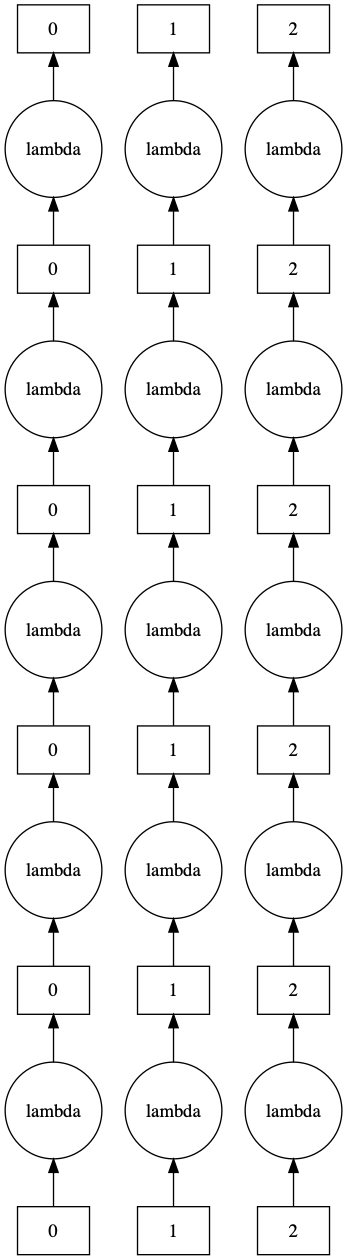
\includegraphics[width=0.125\textwidth,
    angle=-90]{images/incrementation-task-graph.png}
    \caption{Task graph for Incrementation with 5 iterations, represented
    for 3 BigBrain blocks. Circles represent the incrementation and sleep
    function while rectangles represent image blocks.}\label{fig:tg-inc}
\end{figure}

\subsubsection{Histogram}

 Our second application calculates the histogram of the BigBrain image (see
 Algorithm~\ref{alg:histogram}). It reads the image blocks from the shared
 file system, calculates intensity frequencies, aggregates the frequencies
 across the blocks, and finally writes the resulting histogram to the
 shared file system as a single \TG{X}KB file. This application implements
 a typical map-reduce pattern, where the final result is obtained from all
 the input blocks (see Fig.~\ref{fig:tg-histo}). This application requires
 data shuffling thus inter-worker communication. The total amount of shuffled
 data is however limited to \TG{X}MB as it only consists of image
 histograms.

 \TG{Add links to the Github repo for applications and any other relevant file.}

\begin{algorithm}[!t]
    \caption{Histogram}\label{alg:histogram}
    \begin{algorithmic}
    \Require{\(files\), files containing BigBrain}
    \Require{\(fs\), NFS to save image to.}
    \ForEach{\(file \in files\)}
        \State{Read \(block\) from \(file\)}
        \State{{Calculate \(frequency\) of \(blocks\)}}
    \EndFor
    
    \State{\(histogram\gets\)Aggregate \(frequency\) of each \(file\)}

    \State{Write \(histogram\) to \(fs\)}
    \end{algorithmic}
\end{algorithm}

\begin{figure}[!t]
    \centering
    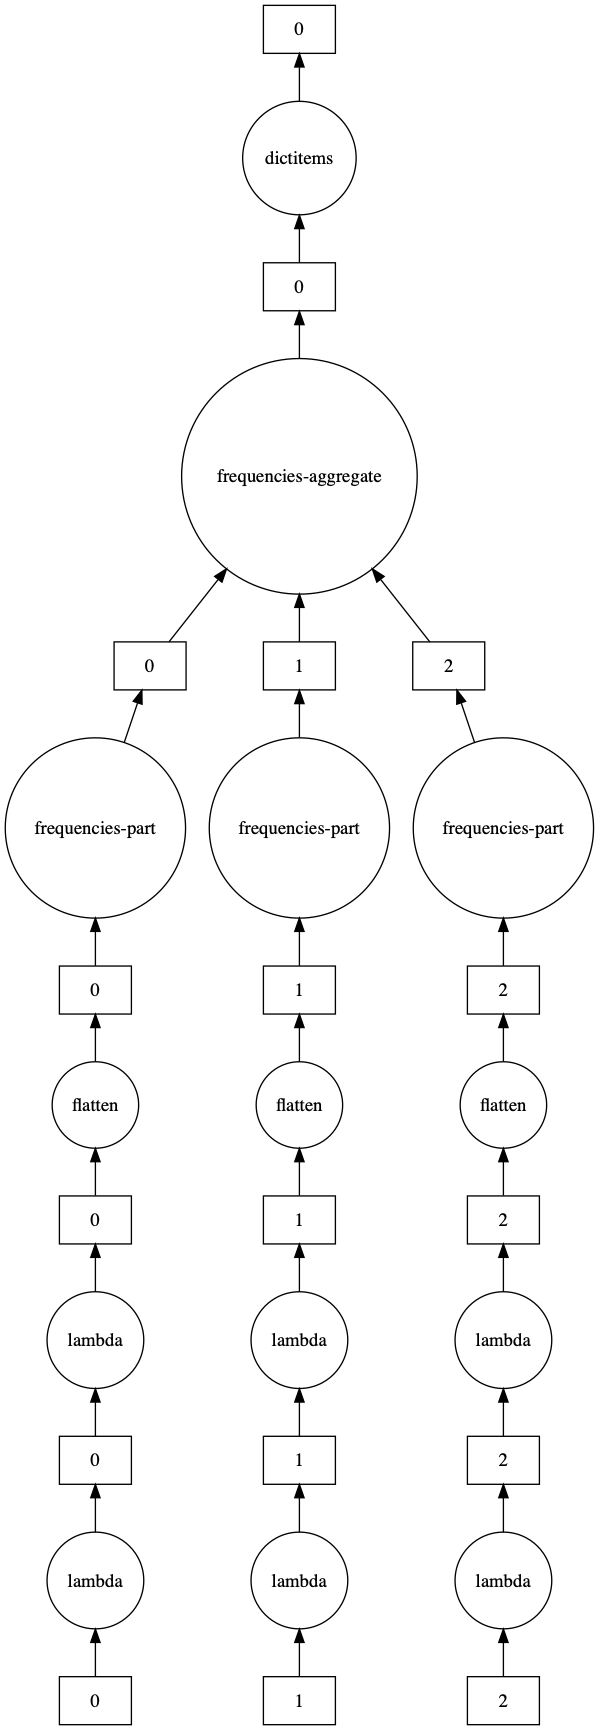
\includegraphics[width=0.16\textwidth, angle=-90]{images/histogram-task-graph.png}
    \caption{Task graph for Histogram}\label{fig:tg-histo}
\end{figure}

\subsubsection{BIDS app example}

We used the \href{https://github.com/BIDS-Apps/example}{BIDS app example}
application available on GitHub. This application operates in a map-reduce
way. The map phase, also called participant analysis, extracts the brain
tissues of a subject's 3D MRI using the popular FMRIB Software Library
(\href{https://fsl.fmrib.ox.ac.uk/fsl/fslwiki}{FSL}), and writes the
resulting image (\TG{X}MB on average) to the shared file system. The reduce
phase, also called group analysis, computes the volume of each brain and
returns the average volume, shuffling a total of \TG{X}GB image data.

While Incrementation and Histogram were implemented directly in Python,
BIDS app example requires an external library and is distributed as a
Docker container image (bids/base\_fsl on DockerHub). To avoid remote file
transfers from DockerHub, we preloaded our OpenStack instances with the
Docker image, and started the Docker engine at startup. \TG{explain run.py modifications if relevant.}

\subsection{Experiments}

We varied four parameters in our experiments, as shown in
Table~\ref{tab:param}. We varied (1) the number of workers to assess the
scalability of the engines, (2) the number of BigBrain blocks in
Incrementation and Histogram to measure the effect of different IO patterns
and parallelization degrees, and (3) the number of iterations and sleep
delay in Incrementation to evaluate the effect of job length.

% The baseline for our experiments is: 8 workers, 125 blocks, 10 iterations and 4
% seconds sleep delay.

\begin{table}[!t]
    \renewcommand{\arraystretch}{1.3}
    \caption{Parameters for the experiments}\label{tab:param}
    \centering
    \begin{tabular*}{\columnwidth}{llll}
    \hline
                        & Incrementation & Histogram             & BIDS Example          \\ \hline
    \# of worker        & 1, 2, 4, 8     & 1, 2, 4, 8            & 1, 2, 4, 8            \\
    \# of blocks        & 30, 125, 750   & 30, 125, 750          & 30, 125, 750          \\
    \# of iterations    & 1, 10, 100     & \multicolumn{1}{c}{-} & \multicolumn{1}{c}{-} \\
    Sleep delay {[}s{]} & 1, 4, 16, 64   & \multicolumn{1}{c}{-} & \multicolumn{1}{c}{-} \\ \hline
    \end{tabular*}
    \end{table}






%%%%% RESULTS %%%%%
\section{Results}

%%% INCREMENTATION %%%
%% worker
\subsection{Experiment 1: Number of workers}
Figure~\ref{fig:inc_ms_worker} shows the makespan for the incrementation algorithm on
the y-axis and the number of workers on the x-axis; the color represents the
different frameworks. Overall, there is no substantial makespan difference between
the frameworks. Also, the increase in performance is not proportional to the number
of workers; performance even decreases when we reach 8 workers.

In Figure~\ref{fig:inc_tt_worker}, the y-axis shows the total execution time of the
incrementation application. The hatch indicates the total time spent for: read,
compute, write, and overhead. Again, the color represents the frameworks. The
computing time stays similar when the number of workers increases. However, the IO
time and overhead increase proportionally to the number of workers.

\begin{figure}[!b]
    \centering
    \begin{subfigure}[b]{\columnwidth}
        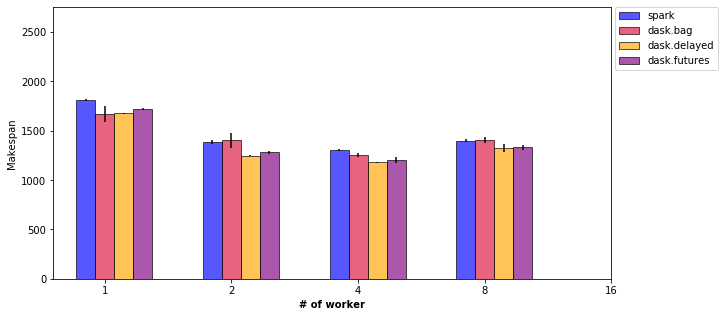
\includegraphics[clip,width=\columnwidth]{images/inc_worker.png}%
        \caption{Incrementation makespan}\label{fig:inc_ms_worker}
    \end{subfigure}
    \\
    \begin{subfigure}[b]{\columnwidth}
        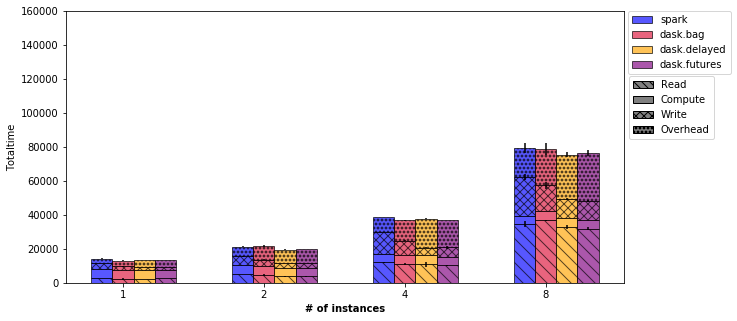
\includegraphics[clip,width=\columnwidth]{images/inc_idle_worker.png}%
        \caption{Incrementation total time}\label{fig:inc_tt_worker}
    \end{subfigure}
    \caption{125 blocks, 10 iterations, 4 sec.\ sleep delay}\label{fig:inc_worker}
\end{figure}

% blocks
\subsection{Experiment 1: Number of blocks}
In Figure~\ref{fig:inc_block}, Spark is not compared for 30 blocks. This is because
Spark has a 2GB limitation in the task size it can compute.

The Figure~\ref{fig:inc_ms_block} shows the makespan evolution when varying the
number of blocks. The compute time increase when there are more blocks. This is
because the sleep delay is constant throughout this experiment and there are more
compute tasks when the number of blocks increases.

In Figure~\ref{fig:inc_tt_block}, the total execution time of each function is shown.
For 30 blocks the Dask Bag API has a much lower overhead time. This is because we
only calculate the idle time of the used core. Dask Bag was only using one thread per
block in comparison to Dask Delayed and Dask Futures which was offloading a block
calculations on multiple threads of the same worker. Furthermore, the variance of the
overhead increases proportionally to the number of blocks. Also, the IO time reduces
with more blocks however the overhead time increase by a similar amount. This is not
observed for 30 blocks as the workers are not used at full capacity; i.e.\ some
threads are idle.

\begin{figure}[!t]
    \centering
    \begin{subfigure}[b]{\columnwidth}
        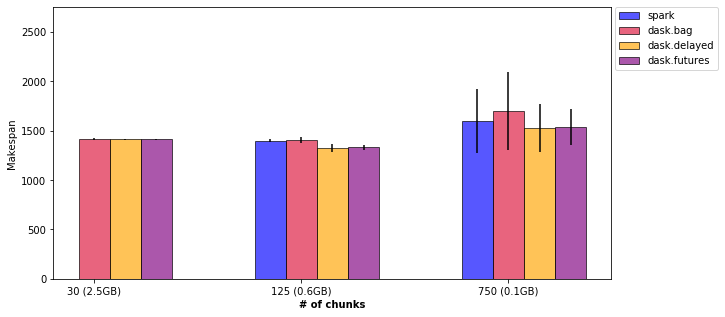
\includegraphics[clip,width=\columnwidth]{images/inc_block.png}%
        \caption{Incrementation makespan}\label{fig:inc_ms_block}
    \end{subfigure}
    \\
    \begin{subfigure}[b]{\columnwidth}
        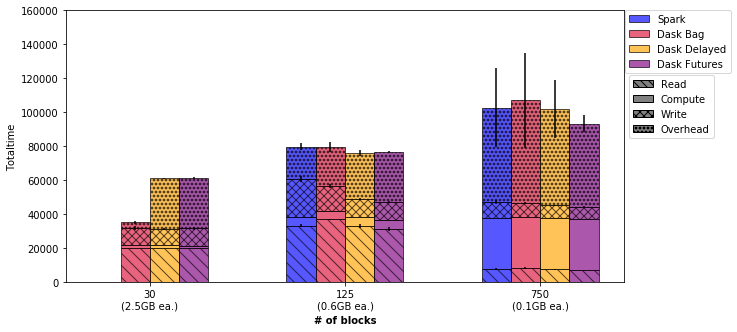
\includegraphics[clip,width=\columnwidth]{images/inc_idle_block.png}%
        \caption{Incrementation total time}\label{fig:inc_tt_block}
    \end{subfigure}
    \caption{10 iterations, 4 sec.\ sleep delay, 8 instances}\label{fig:inc_block}
\end{figure}

%% Iterations
\subsection{Experiment 1: Number of iterations}
Figure~\ref{fig:inc_ms_itr} shows the makespan of the application for the various
number of iterations. Spark and the Dask Bag API are equivalent in terms of
performance. The Dask Delayed API is slightly faster with few iterations (tasks) but
it has a similar makespan to Spark and Dask Bag when the number of iterations
increases. Overall, Dask Futures seems to be faster but the difference is not
substantial.

In Figure~\ref{fig:inc_tt_itr}, the execution time of the function type is shown. The
compute time increase proportionally to the number of iterations. This is because
each computing task has a constant sleep delay. Also, the overhead increases when the
number of iterations (tasks) increases while the IO time decreases; however this is
not substantial.

% We think this is because Dask Delayed often
% schedule a block on a different thread of the same worker which causes small delays
% every time due to inter-thread data communication. This is good when there are fewer
% tasks as is make the IO between blocks go out of sync hence lowering the IO
% bottleneck however as the number of tasks increases those small delays become
% significant.

%  The Dask Futures API seems to outperform all the other APIs but this is
% most likely because the tasks are not interdependent thus this application benefits
% from the less optimal but faster scheduling brought by Dask Futures.

\begin{figure}[!t]
    \centering
    \begin{subfigure}[b]{\columnwidth}
        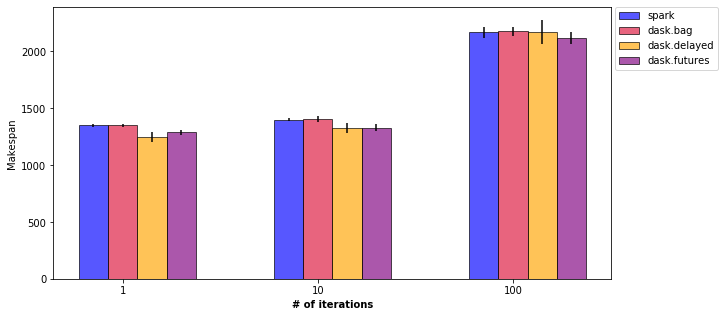
\includegraphics[clip,width=\columnwidth]{images/inc_itr.png}%
        \caption{Incrementation makespan}\label{fig:inc_ms_itr}
    \end{subfigure}
    \\
    \begin{subfigure}[b]{\columnwidth}
        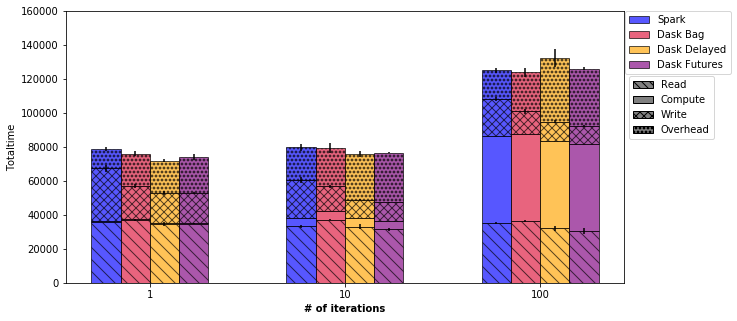
\includegraphics[clip,width=\columnwidth]{images/inc_idle_itr.png}%
        \caption{Incrementation total time}\label{fig:inc_tt_itr}
    \end{subfigure}
    \caption{125 blocks, 4 sec.\ sleep delay, 8 instances}
\end{figure}


%% Sleep time
\subsection{Experiment 1: Sleep delay}
Figure~\ref{fig:inc_ms_sleep} shows the makespan of the incrementation algorithm for
different sleep delays. Spark is initially slower than the Dask APIs, however, it is
faster when increasing the sleep delay. Also, within the Dask APIs, Dask Bag is
slower than the other two but it is not considerable.

Figure~\ref{fig:inc_tt_sleep} shows the execution time for each type of function. On
one hand, Spark has the smallest overhead. Table~\ref{tab:inc_sleep_overhead} shows
that it is substantial; especially with a 64 seconds sleep delay. On the other hand,
Spark has a high IO time. In contrast, Dask Delayed and Futures have the largest
overhead time but the smallest IO time. Then, Dask Bag stands in the middle for both
overhead and IO time.

\begin{table}[!t]
    \caption{Function time for the sleep experiment}
    \begin{subtable}[b]{\columnwidth}
        \renewcommand{\arraystretch}{1.3}
        \caption{Overhead time in second}\label{tab:inc_sleep_overhead}
        \centering
        \begin{tabular}{lllll}
        \hline
                     & 1 sec. & 4 sec. & 16 sec. & 64 sec. \\ \hline
        Spark        & 14992  & 17076  & 16069   & 9769    \\
        Dask.Bag     & 20690  & 21388  & 17759   & 18720   \\
        Dask.Delayed & 27481  & 26199  & 22080   & 24624   \\
        Dask.Futures & 27069  & 27984  & 23538   & 24762   \\ \hline
        \end{tabular}
    \end{subtable}
    \vskip 0.2cm
    \begin{subtable}[b]{\columnwidth}
        \renewcommand{\arraystretch}{1.3}
        \caption{IO time in second}\label{tab:inc_sleep_io}
        \centering
        \begin{tabular}{lllll}
        \hline
                     & 1 sec. & 4 sec. & 16 sec. & 64 sec. \\ \hline
        Spark        & 63622  & 57144  & 51070   & 57078   \\
        Dask.Bag     & 54630  & 52312  & 53743   & 53612   \\
        Dask.Delayed & 45239  & 44142  & 45133   & 46198   \\
        Dask.Futures & 46537  & 43161  & 44749   & 45846   \\ \hline
        \end{tabular}
    \end{subtable}
    \vspace{-3mm}
 \end{table}

\begin{figure}[!t]
    \centering
    \begin{subfigure}[b]{\columnwidth}
        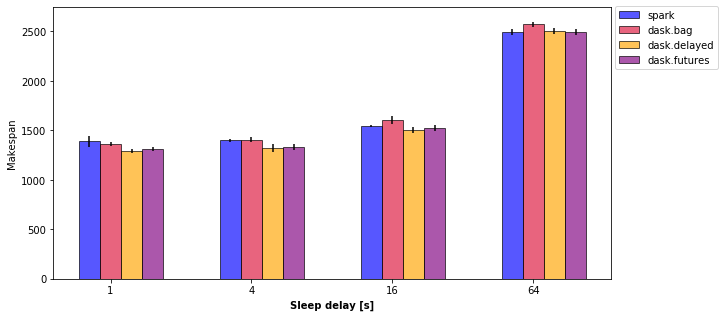
\includegraphics[clip,width=\columnwidth]{images/inc_sleep.png}%
        \caption{Incrementation makespan}\label{fig:inc_ms_sleep}
    \end{subfigure}
    \\
    \begin{subfigure}[b]{\columnwidth}
        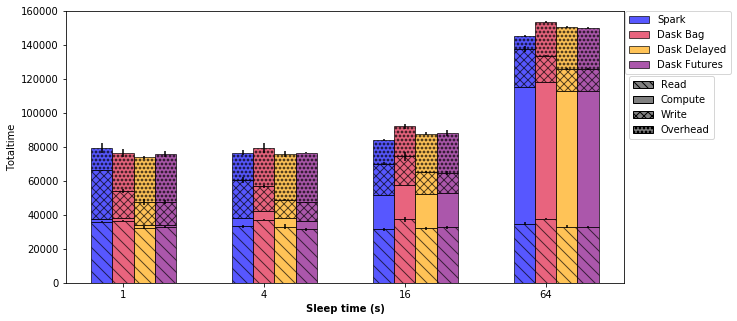
\includegraphics[clip,width=\columnwidth]{images/inc_idle_sleep.png}%
        \caption{Incrementation total time}\label{fig:inc_tt_sleep}
    \end{subfigure}
    \caption{125 blocks, 10 iterations, 8 instances}
\end{figure}

%% Baseline gantt chart
\subsection{Experimentation 1: Baseline timeline}
Figure\ref{fig:inc_gantt} shows the tasks timeline for each worker thread. On the
x-axis is the time in seconds and on the y-axis is the workers and their threads. The
color represents the type of different tasks; note that the color differs from one
graph to another. The first section of reading tasks is much larger than the
following ones. This is because, initially, the NFS is saturated by the number of
workers accessing it. Also, a substantial amount of overhead happens near the IO
tasks. Moreover, for the computing tasks, there is more overhead for the latter tasks.

% The frameworks have similar makespan however the time spend for each type of
% task differs considerably (see Table~\ref{tab:inc_base}). Spark tends to spend more
% time than other frameworks for IO however it has a much lower overhead. Dask Delayed
% and Futures have the lowest IO time but a much higher overhead. Dask Bag stands in
% the middle for both IO and overhead. Compute time is approximately the same for all
% frameworks. Apart from the first IO section, there is a large amount of ovehead
% everytime time IO is performed. This is true for all frameworks.

\begin{figure*}[!htb]
    \centering
    \begin{subfigure}[b]{\columnwidth}
        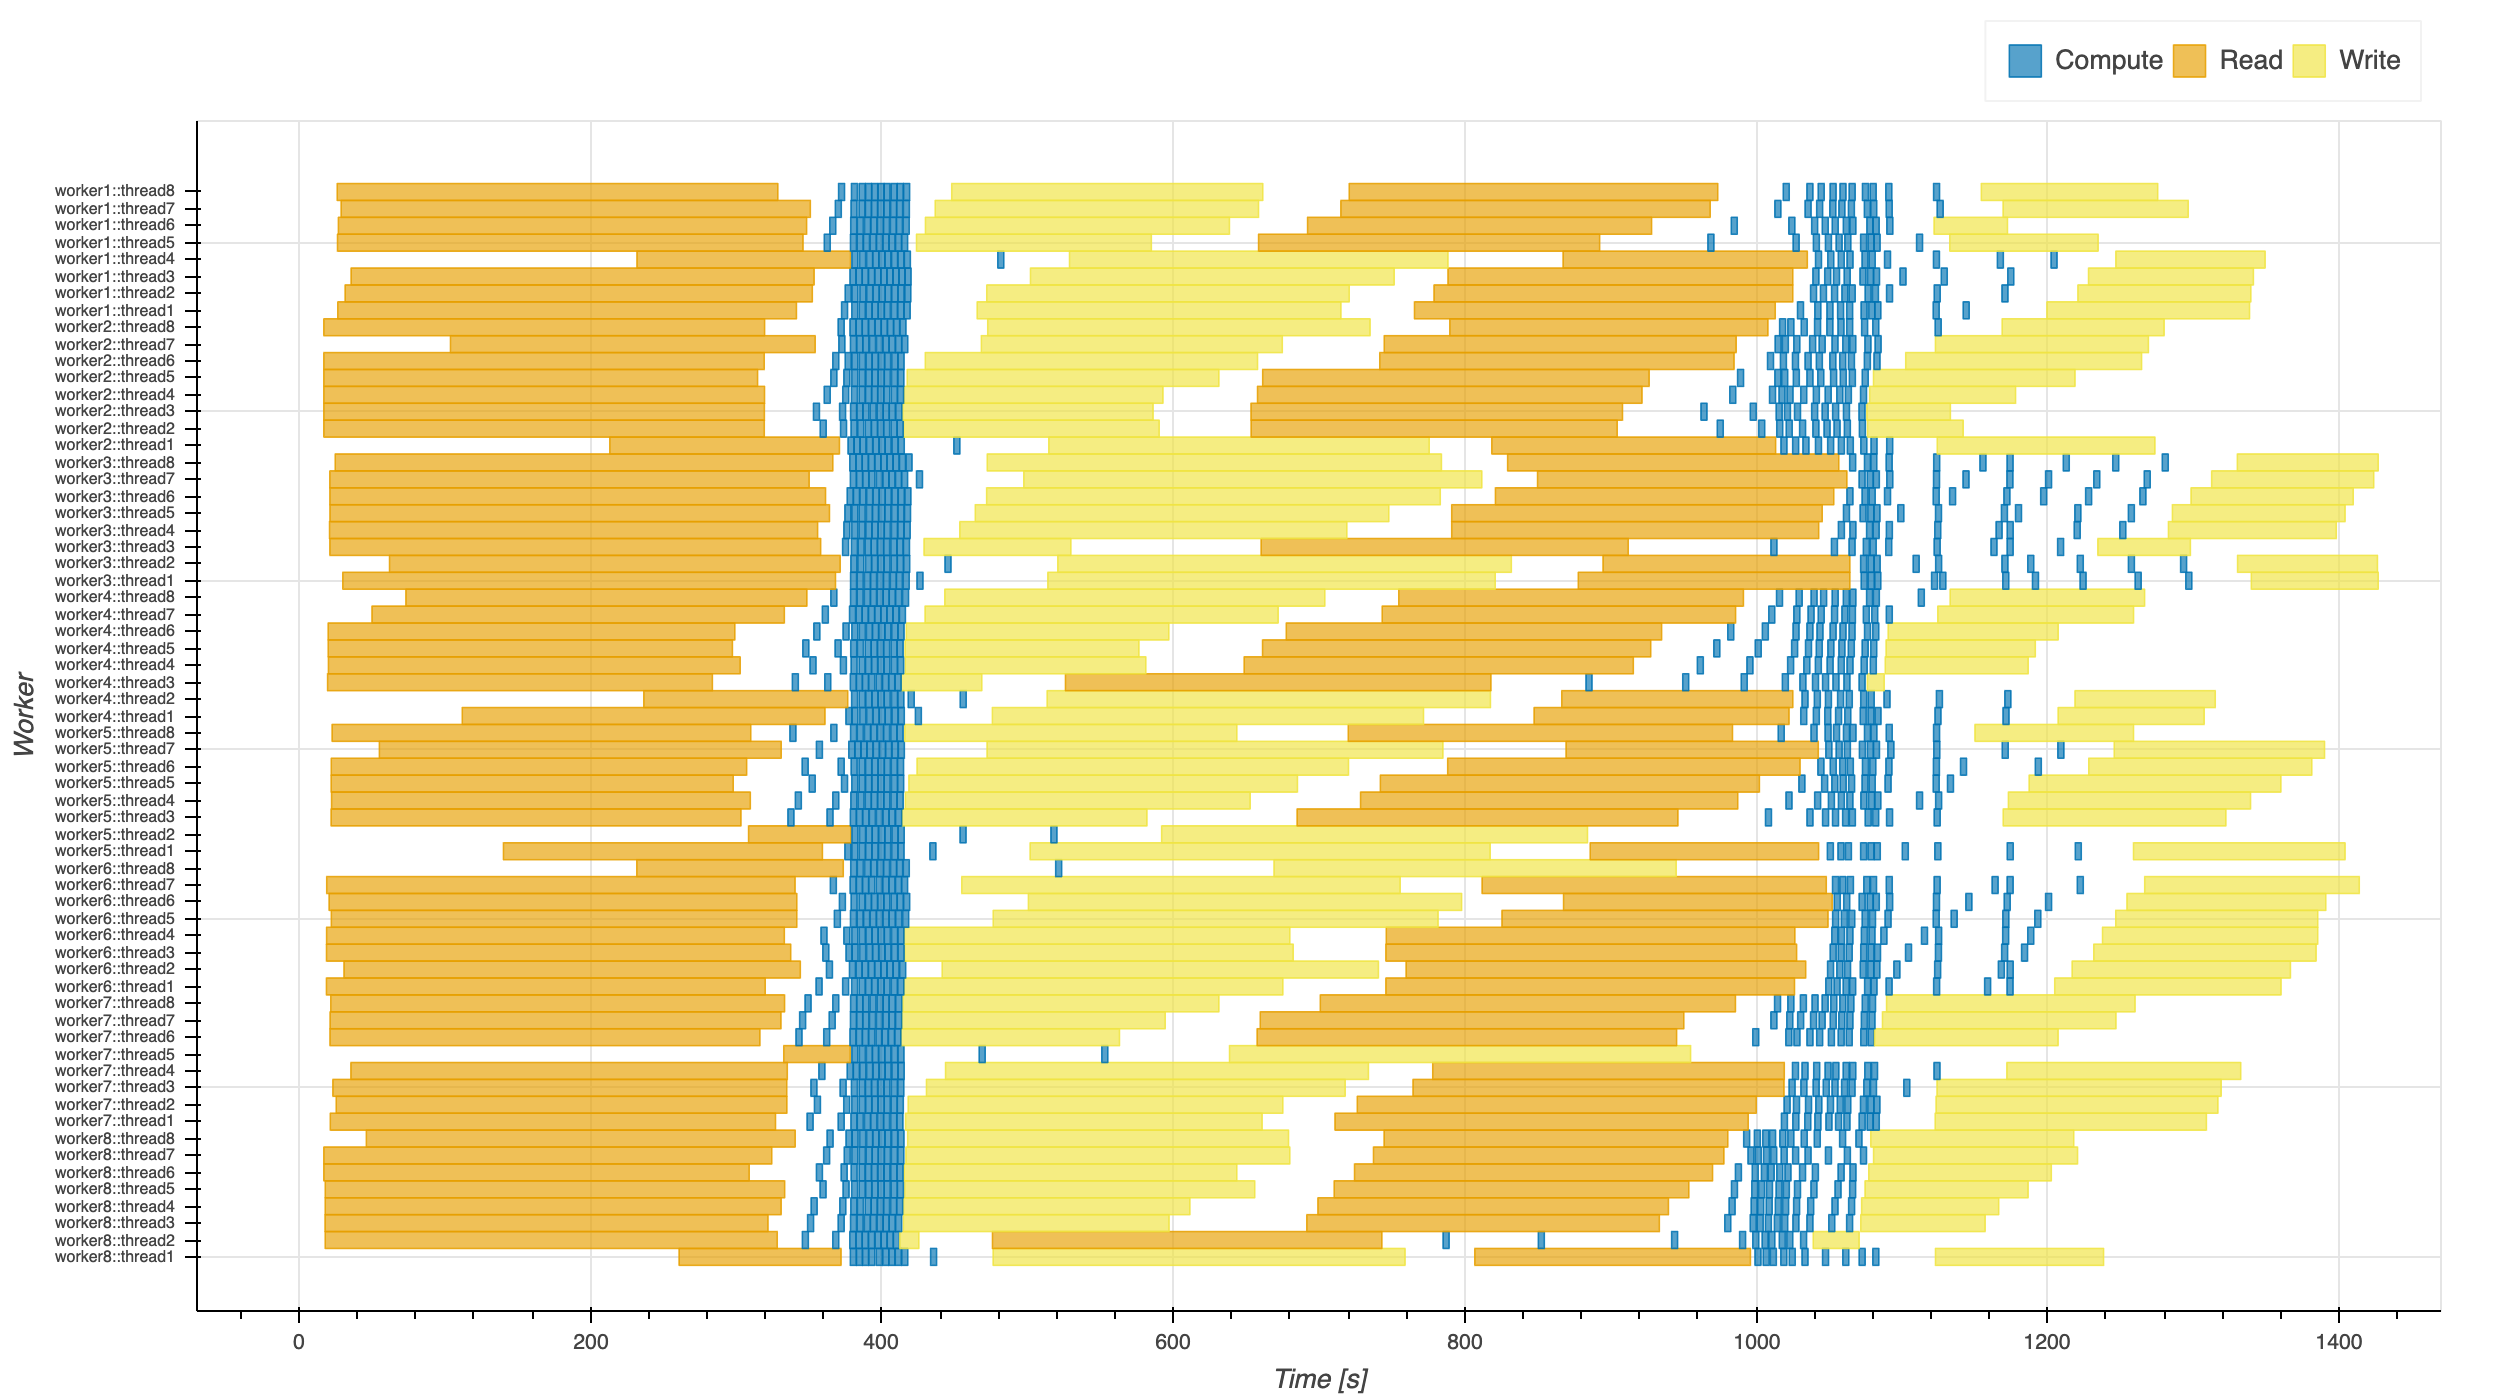
\includegraphics[clip,width=\columnwidth]{images/spark_inc_baseline_gantt.png}
        \caption{Spark execution timeline}\label{fig:inc_spark_gantt}
    \end{subfigure}
    \hfill
    \begin{subfigure}[b]{\columnwidth}
        \includegraphics[clip,width=\columnwidth]{images/Dask_bag_inc_baseline_gantt.png}%
        \caption{Dask Bag execution timeline}\label{fig:inc_dask_bag_gantt}
    \end{subfigure}
    \\
    \begin{subfigure}[b]{\columnwidth}
        \includegraphics[clip,width=\columnwidth]{images/Dask_delayed_inc_baseline_gantt.png}%
        \caption{Dask Delayed execution timeline}\label{fig:inc_dask_delayed_gantt}
    \end{subfigure}
    \hfill
    \begin{subfigure}[b]{\columnwidth}
        \includegraphics[clip,width=\columnwidth]{images/Dask_futures_inc_baseline_gantt.png}%
        \caption{Dask Futures execution timeline}\label{fig:inc_dask_futures_gantt}
    \end{subfigure}
    \caption{125 blocks, 4 sec.\ sleep delay, 8 instances}\label{fig:inc_gantt}
\end{figure*}

% \begin{table}[!b]
%     \renewcommand{\arraystretch}{1.3}
%     \caption{Distribution of the execution time in second: 125 blocks, 4 sec.\ sleep
%     delay, 10 iterations, and 8 workers}\label{tab:inc_base}
%     \centering
%     \begin{tabular*}{\columnwidth}{llllll}
%     \hline
%                  & Read  & Compute & Write & Overhead & Total \\ \hline
%     Spark        & 34465 & 5118    & 22679 & 17076    & 79338 \\
%     Dask Bag     & 36863 & 5121    & 15449 & 21388    & 78821 \\
%     Dask Delayed & 32769 & 5119    & 11373 & 26199    & 75461 \\
%     Dask Futures & 31891 & 5120    & 11270 & 27984    & 76265 \\ \hline
%     \end{tabular*}
%  \end{table}

%%% HISTOGRAM %%%
\subsection{Experiment 2: Number of instances}

\begin{figure}[!t]
    \centering
    \begin{subfigure}[b]{\columnwidth}
        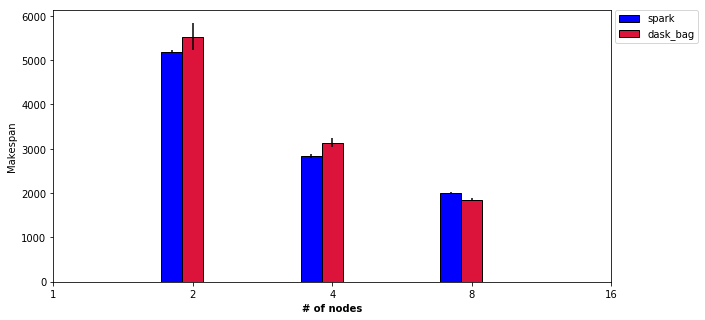
\includegraphics[clip,width=\columnwidth]{images/histo_instance.png}%
        \caption{Histogram makespan}\label{fig:histo_ms_worker}
    \end{subfigure}
    \\
    \begin{subfigure}[b]{\columnwidth}
        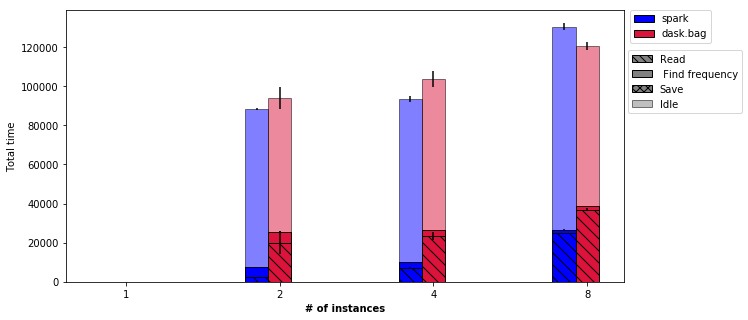
\includegraphics[clip,width=\columnwidth]{images/histo_idle_instances.png}%
        \caption{Histogram total time}\label{fig:histo_tt_worker}
    \end{subfigure}
    \caption{125 blocks}
\end{figure}

\subsection{Experiment 2: Number of blocks}

\begin{figure}[!t]
    \centering
    \begin{subfigure}[b]{\columnwidth}
        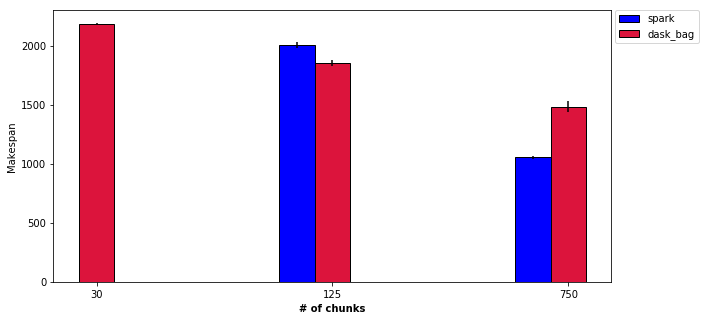
\includegraphics[clip,width=\columnwidth]{images/histo_splits.png}%
        \caption{Histogram makespan}\label{fig:histo_ms_block}
    \end{subfigure}
    \\
    \begin{subfigure}[b]{\columnwidth}
        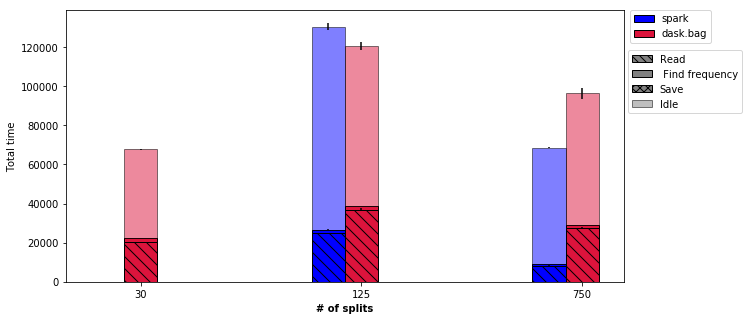
\includegraphics[clip,width=\columnwidth]{images/histo_idle_splits.png}%
        \caption{Histogram total time}\label{fig:histo_tt_block}
    \end{subfigure}
    \caption{8 workers}
\end{figure}
\TG{We decided to omit Dask Futures as it does not have any value over Dask
Delayed in this application.}
%%% BIDS EXAMPLE %%%
\subsection{Experiment 3: Number of instances}



%%%%% DISCUSSION %%%%%
\section{Discussion}
\subsection{IO Time}


\subsection{Serialization}
We think that serialization could have an important effect on the makespan of the
application. This could potentially slow down the application when a lot of tasks are
scheduled.

\subsection{NFS}
The NFS seems to be a source of the bottleneck. We think that exploring another file
system, like Lustre, could give us insight into the actual effect of the NFS on the
application makespan. We also think that the NFS caching could play an effect on the
task of different lengths.

\subsection{Scheduler}
The Dask scheduler seems to have some bizarre behavior. It seems like it waits to
schedule tasks. It could also be due to tasks being scheduled on other workers
thus requiring data to be sent over the network; which would explain the stall on the
worker. More work would be needed to investigate that issue.


\subsection{Caching}
We think that caching plays an effect on the results. As seen in the Gantt chart
previously, some of the read tasks are significantly shorter than others while all
blocks are of equal size.

\section*{Acknowledgment}

Mathieu Dugr\'e was funded by a Undergraduate Summer Research Assistant
award from the National Science and Engineering Research Council. We warmly
thank Compute Canada and \TG{Westgrid?} for providing the cloud
infrastructure used in these experiments, and the McGill Center for
Integrative Neurocience for giving us access to their cloud allocation.

\bibliographystyle{IEEEtran}
\bibliography{IEEEabrv,reference}

\end{document}
